\section{Introduction}
Location-based social network services allow users to perform check-in and share their check-in data with their friends. In particular, when a user is traveling, the check-in data are in fact a travel trajectory with some photos and tag information. As a result, a massive number of trajectories are generated, which play an essential role in many well-established research areas, such as mobility prediction, urban planning and traffic management. In this paper, we focus on trip planning and intend to discover travel experiences from shared data in location-based social networks. To facilitate trip planning, the prior works in \cite{SIGMOD2010}\cite{hsieh2014mining}\cite{ICPADS2007}\cite{skyline2014}\cite{WWW2009} provide an interface in which a user could submit the query region and the total travel time. In contrast, we consider a scenario where users specify their preferences with keywords. For example, when planning a trip in Sydney, one would have ``Opera House''. As such, we extend the input of trip planning by exploring possible keywords issued by users. However, the query results of existing travel route recommendation services usually rank the trajectories simply by the popularity or the number of uploads of trajectories. 

For such ranking, existing works~\cite{yuan2014graph}\cite{ye2011exploiting}\cite{ytwen2014} derive a scoring function, and each trajectory will have one score according to its features (e.g., the number of Places of Interest, the popularity of places). Usually, the query results will have similar trajectories. In contrast, this work considers the diversity of results, as high scoring trajectories are often too similar to each other. Our goal is to retrieve a greater diversity of trajectories based on the travel factors considered.

 % Typically, a trajectory is a sequence of geo-locations with time-stamps, and a travel route may pass through a sequence of places of interest (POIs). Obviously, users would like to acquire travel routes that contains a set of POIs instead of individual ones. Note that every POI has its' proper visiting time. For example, people would like to go to night market in the night because there has a lot of vendors and people can enjoy their shopping and food travel. On the contrary, night market may have no venders and nothing interesting if people visit it in the day time. Furthermore, users may have some personalized requirements like must-visit POI(s) to be added into their trip plan. For instance, Tim wants to have a one day trip in Melbourne and he want to visit Federation Square. It would be helpful if a travel route recommendation system is able to recommend trips that contain Federation Square and some nearby interesting regions in Melbourne. Addition information can also be explored from geo-social network to find out influential friends, e.g., assume Tim always refer Kelly for travel tips, Tim would probably be interest in the travel itinerary Kelly has. % There are many representative work includes trajectory search frameworks \cite{SIGMOD2010,hsieh2014mining,ICPADS2007,skyline2014,WWW2009} mining knowledge form trajectories \cite{yuan2014graph,ye2011exploiting,ytwen2014}, and efficient search algorithms \cite{SIGMOD2010,ICDE2013,cao2012keyword} are proposed in these years. 

\begin{figure}[t]
\centering
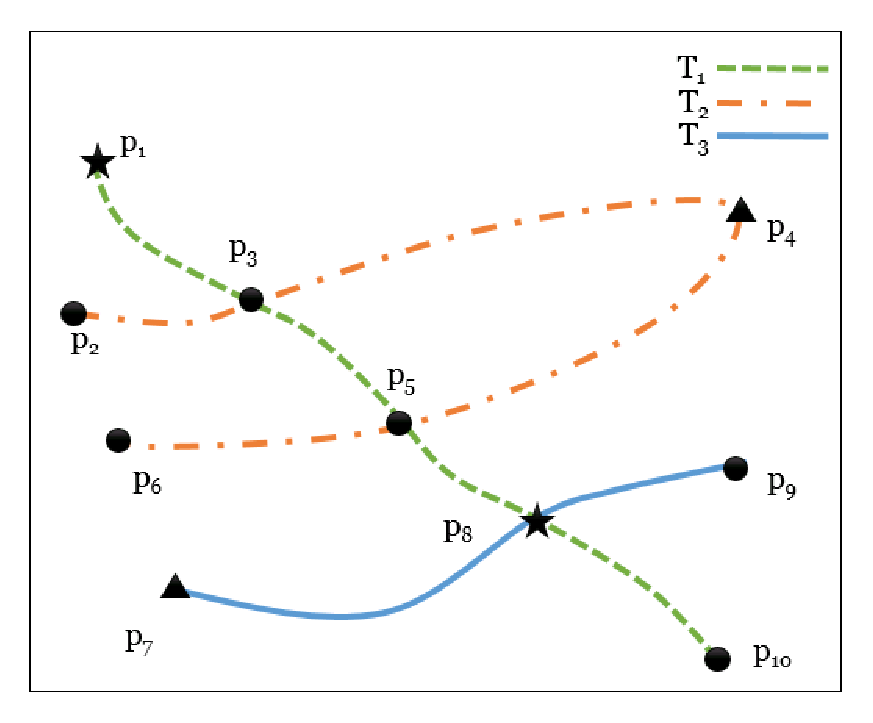
\includegraphics[width=6cm]{intro_example.eps}
\caption{Keyword-aware travel routes query running example.}
\label{fig:running_example}
\end{figure}

\begin{table}[t]
 \centering
 \caption{Example of trajectory dataset}
 \begin{footnotesize}
 \begin{tabular}{|c|l|l|l|l|l|} \hline
 Tid & Uid & Pid & keyword & time & POI score vector\\ \hline
 $T_{1}$ & $u_{1}$ & $p_{1}$ & Opera House & 10:00 & (0.04, 0.2) \\ \hline
 $T_{1}$ & $u_{1}$ & $p_{3}$ & Bar & 12:00 & (0.25, 0.2) \\ \hline
 $T_{1}$ & $u_{1}$ & $p_{5}$ & Bar & 15:30 & (0.2, 0.8) \\ \hline
 $T_{1}$ & $u_{1}$ & $p_{8}$ & Opera House & 17:30 & (0.04, 0.3) \\ \hline
 $T_{1}$ & $u_{1}$ & $p_{10}$ & Bar & 19:00 & (0.04, 0.2) \\ \hline
 $T_{2}$ & $u_{2}$ & $p_{2}$ & Bar & 10:30 & (0.02, 0.2) \\ \hline
 $T_{2}$ & $u_{2}$ & $p_{3}$ & Bar & 12:30 & (0.25, 0.2) \\ \hline
 $T_{2}$ & $u_{2}$ & $p_{4}$ & Sunset & 17:00 & (0.05, 0.2) \\ \hline
 $T_{2}$ & $u_{2}$ & $p_{5}$ & Bar & 19:00 & (0.2, 0.8) \\ \hline
 $T_{2}$ & $u_{2}$ & $p_{6}$ & Bar & 19:30 & (0.25, 0.8) \\ \hline
 $T_{3}$ & $u_{3}$ & $p_{7}$ & Sunset & 18:30 & (0.4, 0.8) \\ \hline
 $T_{3}$ & $u_{3}$ & $p_{8}$ & Opera House & 19:30 & (0.04, 0.3) \\ \hline
 $T_{3}$ & $u_{3}$ & $p_{9}$ & Bar & 20:00 & (0.1, 0.1) \\ \hline
 \end{tabular}
 \end{footnotesize}
 \label{Tab:intro_tra}
 \vspace{-5mm}
 \end{table}

In this paper, we develop a Keyword-aware Skyline Travel Route (\textit{KSTR}) framework to retrieve several recommended trajectories where keyword means the personalized requirements users have for the trip. Consider an example illustrated in Figure \ref{fig:running_example}, the related route information of which is stored in Table \ref{Tab:intro_tra}. For ease of illustration, each POI is associated with one keyword (though our model can support multiple keywords) and a two-dimensional score vector (each dimension repersents the rank of a feature). Assume a tourist plans a date with a set of keywords [``Whisky'' ``Sydney Cove'' ``Sunset'']. First, we can find that these keywords vary in their semantic meaning: ``Sydney Cove'' is a geographical region; ``Sunset'' is related to a specific time period (evening) and locations such as beach; ``Whisky'' is the attribute of POI. 

We argue knowing semantics is important, as some query keywords do not need to be matched in POI keyword. For example, $p_9$, even though its name does not include ``Whiskey'', is a good match, as it is an important attribute of Bar POIs.  Similarly, ``Sydney Cove'' is not mentioned, but based on the location of Opera House, $p_8$ matches the requirement. As a result, $T_3$ matches all the requirements, which could not be supported by existing simple keyword-based matches.%In this example, the keyword ``Sunset'' can be easily matched. Although the other two words are not stored in the database, we want to correspond them to \textit{Drinking whisky at bar} and \textit{Opera House in Sydney Cove}. Finally, $T_3$ matches all the requirements. Meanwhile, there is still a possibility that no existing trajectory is in accordance with the query keywords. For this challenge, we propose a candidate route generation algorithm to increase the number of trajectories. For instance, a travel sequence $T'=\{p_1\rightarrow p_3\rightarrow p_4\rightarrow p_5\rightarrow p_8\rightarrow p_9\}$, which is aggregated from trajectory segments of $T_1$ to $T_3$, also matches all the keywords specified.

With a set of travel routes, feature scoring should be considered to find proper recommendations. We explore three travel factors: ``Where: people tend to visit popular POIs'', ``When: each POI has its proper visiting time'', and ``Who: people might follow social-connected friends' footsteps''. In the view of POI, we store the attractiveness score and the visiting time information in the POI score vector. In the view of user, we also consider a score to quantify individual's influence in recommendation.

Additionally, we have mentioned that the final results may have similar characteristics and be monotonous due to that all factoring are aggregated into one score for each travel route. Consequently, the system will retrieve top-1 or top-$K$ trajectories with the highest score as the results. Users may not understand the characteristic of these trajectories through the final one score (e.g., Which one has most interesting landmarks? Which one is well-connected to the place I want to go?) so that it may be hard to choose a trajectory from the final results. Furthermore, user need to pre-defined the weight for each factor although it is hard to select suitable weight in most cases. Since travel route recommendation has to take several factors into consideration to emphasize the unique travel factors of travel routes, we borrow the concept of Skyline to retrieve travel routes. Skyline search on the travel routes retrieves all the possible optimal results in terms of features derived, and hence a diverse set of travel routes is retrieved. Consider an example in Figure~\ref{fig:running_example}, where the score vector of POIs represents the attractiveness score and the visiting time information. To compute the average POI score of $T_1$, $T_2$ and $T_3$, we get the final score values (0.1,0.34), (0.15,0.44), and (0.18,0.3) respectively. The skyline result is $\{T_2,T_3\}$. 

Consequently, in this paper, travel routes have several score values mined from social media. By exploiting Skyline query, a diverse set of travel routes is determined. In addition, travel routes could be constructed from different trajectory segments. We further propose one approximate algorithm to efficiently derive travel routes. % and the best choice is usually from these routes. % Conventional trajectory recommendation systems usually assign a score for each factor and define a weighting score function to aggregate all these scores derived from each factor into one score. The trajectories with the highest score are recommended to users.

The contributions of this paper are summarized as follows:
\begin{itemize}
  \item We propose a \textit{KSTR} framework in which users are able to issue a set of keywords and a query region, and for which query results contain diverse trip trajectories.  
  \item We propose a novel keyword extraction module to extract three types of keywords: Geo-specific keywords, Temporal keywords and Attribute keywords. % the semantic meaning of user-specific keywords.
  \item We extract three travel factors of POIs from LBSNs: attractiveness of POIs, the visiting time of POIs and the geographical social influence. 
  \item We propose a trajectory reconstruction method to partition trajectories into segments by considering spatial and temporal features. % Based on this, we develop a novel method to aggregate the place which user prefer to visit into trajectory and design a scoring function to measure how well the trajectory connect to query points.
  \item Skyline query for travel route search is adopted to combine the multi-dimensional measurements (POI attractiveness, proper visiting time and geographical social influence) of routes, which increase the diversity of the recommended results. 
  \item An approximate algorithm is adopted to derive efficient results for the online interactive system.
\end{itemize}
To evaluate our proposed framework, we conducted experiments on real LBSN and photo datasets. The experimental results show that \textit{KSTR} is able to retrieve travel routes that are of interest to users.

% the following will be revised later
%The rest of the paper is organized as follows. Section 2 presents the overview of the \textit{KSTR} framework. Section 3 describes the feature scoring algorithms. In Section 4, we provide a travel routes exploration module of \textit{KSTR}. Experimental results of proposed method are shown in Section 5. Finally, Section 6 concludes this paper.

